\subsection{Graphs and Networks}
\label{sec:Method:Graphs}
The most common way of describing a network of anything, that could be of accounts on Facebook, the electrical grid, distribution of goods from warehouses to stores etc. is to use a graph.
A graph is a representation of a network that consists of a set of $N$ nodes, the entities whose interactions are being depicted, and edges $E$ which represent said interactions.


\subsubsection{Static Graphs}
\label{sec:Method:Graphs:StaticGraphs}
The most common type of graph is a static graph, providing a representation of the nodes in a network and edges that are static, ie. do not change. 
In this way, the static graph can be seen as a snapshot of a given network at a single point in time.

A static graph representation the relationships between you and three friends who do not know each other could look as presented in figure \ref{fig:StaticGraph}.

\begin{figure}[H]
    \centering
    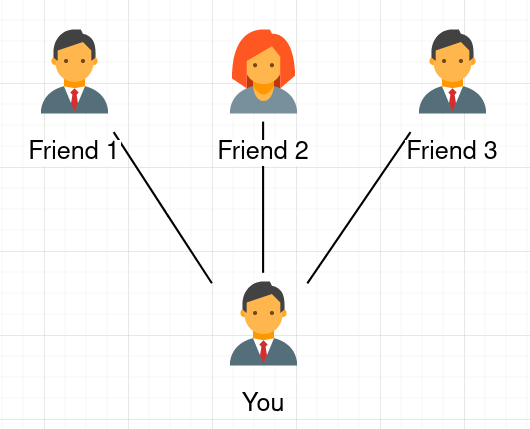
\includegraphics[width=\textwidth]{0_images/static_graph.png}
    \caption{The relationship between you and three friends. You know each one of them, buth they do not know each other.}
    \label{fig:StaticGraph}
\end{figure}


\subsubsection{Temporally Dynamic Graphs}
\label{sec:Method:Graphs:DynamicGraphs}
Not all networks can be represented by static graphs though, and sometimes having graphs be non-static means that they make for a better representation of the network they are modelling. 
When talking about the graphs of a dynamic network, this project refers to graphs that are subject to a sequence of \textit{updates} over time. 
An update is an action that \textit{inserts} or \textit{deletes} edges or nodes in the graph or actions that \textit{alter attributes} of nodes or edges.

The dynamic aspect differ between graphs, as they can be changing in different dimensions. 
This project focuses entirely on the very commonly used graphs that are dynamic in the temporal dimension, \textit{temporal dynamics graphs}, i.e. they change over time, this is not always the case. 

A very simple dynamic network could be visualized by the following 

\begin{figure}[H]
    \centering
    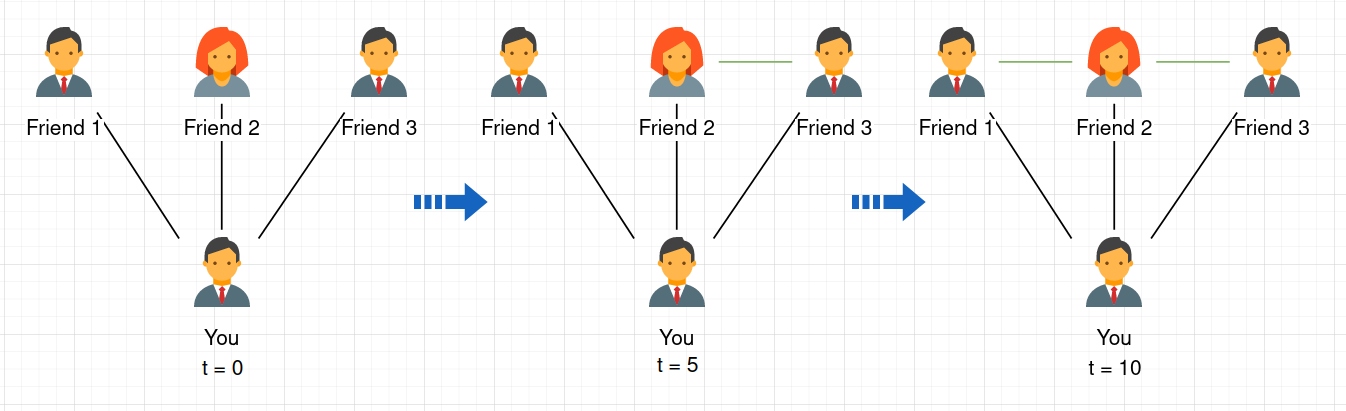
\includegraphics[width=\textwidth]{0_images/dynamic_graph.png}
    \caption{The dynamic relationship between you and three friends, changing from time $t=0$, to time $t=5$ and lastly $t=10$. Between each time, the friends get to know each other, and the graph hence changes over time.}
    \label{fig:StaticGraph}
\end{figure}


Another example could be if we had a network representing the airports which a plane could directly fly to. 
Now the graph would be dynamic in the geographical position of the plane as the graph could change to show which airport the plane is connected to based on its current position. 
Say the graph for the plane being at the Reykjavik Airport on Iceland will then change when the plane gets to Los Angles.










